

\documentclass[man,floatsintext]{apa6}
\usepackage{lmodern}
\usepackage{amssymb,amsmath}
\usepackage{ifxetex,ifluatex}
\usepackage{fixltx2e} % provides \textsubscript
\ifnum 0\ifxetex 1\fi\ifluatex 1\fi=0 % if pdftex
  \usepackage[T1]{fontenc}
  \usepackage[utf8]{inputenc}
\else % if luatex or xelatex
  \ifxetex
    \usepackage{mathspec}
  \else
    \usepackage{fontspec}
  \fi
  \defaultfontfeatures{Ligatures=TeX,Scale=MatchLowercase}
\fi
% use upquote if available, for straight quotes in verbatim environments
\IfFileExists{upquote.sty}{\usepackage{upquote}}{}
% use microtype if available
\IfFileExists{microtype.sty}{%
\usepackage{microtype}
\UseMicrotypeSet[protrusion]{basicmath} % disable protrusion for tt fonts
}{}
\usepackage{hyperref}
\hypersetup{unicode=true,
            pdftitle={Assessing sampling methods for generalization from RCTs: Modeling recruitment and participation},
            pdfauthor={Gleb Furman~\& James E. Pustejovsky},
            pdfborder={0 0 0},
            breaklinks=true}
\urlstyle{same}  % don't use monospace font for urls
\usepackage{graphicx,grffile}
\makeatletter
\def\maxwidth{\ifdim\Gin@nat@width>\linewidth\linewidth\else\Gin@nat@width\fi}
\def\maxheight{\ifdim\Gin@nat@height>\textheight\textheight\else\Gin@nat@height\fi}
\makeatother
% Scale images if necessary, so that they will not overflow the page
% margins by default, and it is still possible to overwrite the defaults
% using explicit options in \includegraphics[width, height, ...]{}
\setkeys{Gin}{width=\maxwidth,height=\maxheight,keepaspectratio}
\IfFileExists{parskip.sty}{%
\usepackage{parskip}
}{% else
\setlength{\parindent}{0pt}
\setlength{\parskip}{6pt plus 2pt minus 1pt}
}
\setlength{\emergencystretch}{3em}  % prevent overfull lines
\providecommand{\tightlist}{%
  \setlength{\itemsep}{0pt}\setlength{\parskip}{0pt}}
\setcounter{secnumdepth}{0}
% Redefines (sub)paragraphs to behave more like sections
\ifx\paragraph\undefined\else
\let\oldparagraph\paragraph
\renewcommand{\paragraph}[1]{\oldparagraph{#1}\mbox{}}
\fi
\ifx\subparagraph\undefined\else
\let\oldsubparagraph\subparagraph
\renewcommand{\subparagraph}[1]{\oldsubparagraph{#1}\mbox{}}
\fi

%%% Use protect on footnotes to avoid problems with footnotes in titles
\let\rmarkdownfootnote\footnote%
\def\footnote{\protect\rmarkdownfootnote}


  \title{Assessing sampling methods for generalization from RCTs: Modeling
recruitment and participation}
    \author{Gleb Furman\textsuperscript{1}~\& James E.
Pustejovsky\textsuperscript{1}}
    \date{}
  
\shorttitle{Assessing sampling methods for generalization from RCTs}
\affiliation{
\vspace{0.5cm}
\textsuperscript{1} University of Texas at Austin}
\usepackage{csquotes}
\usepackage{upgreek}
\captionsetup{font=singlespacing,justification=justified}

\usepackage{longtable}
\usepackage{lscape}
\usepackage{multirow}
\usepackage{tabularx}
\usepackage[flushleft]{threeparttable}
\usepackage{threeparttablex}

\newenvironment{lltable}{\begin{landscape}\begin{center}\begin{ThreePartTable}}{\end{ThreePartTable}\end{center}\end{landscape}}

\makeatletter
\newcommand\LastLTentrywidth{1em}
\newlength\longtablewidth
\setlength{\longtablewidth}{1in}
\newcommand{\getlongtablewidth}{\begingroup \ifcsname LT@\roman{LT@tables}\endcsname \global\longtablewidth=0pt \renewcommand{\LT@entry}[2]{\global\advance\longtablewidth by ##2\relax\gdef\LastLTentrywidth{##2}}\@nameuse{LT@\roman{LT@tables}} \fi \endgroup}

\usepackage{amsthm}
\newtheorem{theorem}{Theorem}[section]
\newtheorem{lemma}{Lemma}[section]
\theoremstyle{definition}
\newtheorem{definition}{Definition}[section]
\newtheorem{corollary}{Corollary}[section]
\newtheorem{proposition}{Proposition}[section]
\theoremstyle{definition}
\newtheorem{example}{Example}[section]
\theoremstyle{definition}
\newtheorem{exercise}{Exercise}[section]
\theoremstyle{remark}
\newtheorem*{remark}{Remark}
\newtheorem*{solution}{Solution}
\begin{document}
\maketitle

\begin{verbatim}
## Warning: package 'stargazer' was built under R version 3.5.2
\end{verbatim}

\begin{verbatim}
## Warning: package 'htmlTable' was built under R version 3.5.2
\end{verbatim}

\begin{verbatim}
## Warning: package 'Hmisc' was built under R version 3.5.2
\end{verbatim}

\begin{verbatim}
## Warning: package 'Formula' was built under R version 3.5.2
\end{verbatim}

Recently, randomized controlled trials (RCTs) have come under scrutiny
for their limited generalizability due to inadequate sampling strategies
(Stuart, Cole, Bradshaw, \& Leaf, 2011). RCTs provide a high level of
internal validity as they demonstrate the causality of the impact being
estimated. In education research, multisite RCTs, or multisite
randomized trials (MRTs), are used to inform policy decisions by
evaluating intervention impacts on a larger scale. Recruitment and
randomization occurs at the organizational level (e.g.~schools),
ostensibly increasing the diversity of settings in which the study takes
place. In practice, however, the generalizability of MRTs is greatly
limited by the sampling method being implemented. This is a major
drawback for policymakers who are interested in generalizing treatment
effects beyond the sample.

RCTs are commonly used in impact evaluations across many fields.
Randomized treatment assignment ensures that estimated effects are
causal, thus affording a higher level of internal validity. However,
these effect estimates may be sample specific. If treatment effects are
heterogeneous, then the impact of an intervention cannot be extrapolated
beyond the study sample. This is a limiting feature of RCTs since
policymakers seeking to implement interventions will have no way of
gaguing effectivenes in their populaton of interest.

MRTs attempt to remedy this by studying the intervention on a larger
scale. In educational research, for instance, multiple schools may be
recruited to participate in a study, with each school randomly assigned
to receive the intervention or continue buisiness as usual (BAU). This
design offers greater external validity relative to the single-site
variant because it enables the study of site-by-treatment interaction
and formal tests of generaliability (Raudenbush \& Liu, 2000). Treatment
effect estimates are said to be generalizable to schools that are
\enquote{similar} to those in the study, however, the similarity can be
difficult to define. Furthermore, if the sample of sites is too small or
homogeneous, the scope of the generalization is greatly diminished.

Random sampling overcomes this limitation by selecting sites from a
well-defined population with some known probability. When used in
conjunction with randomized treatment assignment, this is known as dual
randomization. Assuming no refusals during recruitment, and full
compliance without attrition after assignment, this design enables
unbiased estimation of the sample average treatment effect (SATE). Using
the known sampling probabilities, the SATE can then be used to estimate
the population average treatment effect (PATE).

In absence of random sampling, PATE can still be estimated by using
propensity score techniques, provided there is sufficent overlap between
the sample and the population (O'Muircheartaigh \& Hedges, 2014; Tipton,
2013a). This is especially usefull in impact evaluation as probability
sampling is rarely used in this context (Olsen, Orr, Bell, \& Stuart,
2013; Shadish, Cook, \& Campbell, 2002). Instead, researchers often opt
for convenience or purposive samples. These methods much less expensive
to implement, but are not usually designed for representative sampling.
This makes them susceptible to undercoverage, or substantial differencs
between the sample and target population (Groves, 2004). Undercoverage
can be assessed using similar propensity score techniques (Stuart et
al., 2011; Tipton, 2014). When undercoverage is too great, the full PATE
cannot be recovered with the given sample, and the population needs to
be trimmed by removing subsets of sites that are not represented.

A series of recent papers instead advocate planning for generalizability
at the recruitment stage (Tipton, 2013a, 2013b). These methods require a
well defined and enumerated population for which there is extant data,
making them especially relevant in the educational context. One method
in particular, Stratified Balanced Sampling (SBS), has attracted
attention from researchers due to its accessibility. The method involves
using cluster analysis to split the population into smaller homogeneous
strata and ranking units within each strata to prioritize for
recruitment in order to achieve a representative sample. Researchers who
are interested in using this to sample schools may even use a website
(www.thegeneralizer.org) which guides them through this process using
data from the Common Core of Data.

Potential advantages of SBS include reducing undercoverage and greater
recruitment transparency. However, little methodological work has
examined this method's effectiveness. Schools and districts with certain
characteristics are unlikely to participate in large-scale MRTs
(Fellers, 2017; Stuart, Bell, Ebnesajjad, Olsen, \& Orr, 2017; Tipton et
al., 2016). If one or more strata are comprised of difficult schools,
researchers may resort to convenience sampling within those strata.
Furthermore, the additional resources required to recruit from all
strata create concerns regarding practicality.

The goal of the current paper is two-part. First, we propose several
methods for modeling two major sources of sampling bias: recruitment and
participation. Recruitment refers to how likely a sampling unit is to be
approached by researchers, and participation refers to how likely the
sampling unit is to participate if recruited. This step will lay the
groundwork for testing sampling methods in the educational context.
Second, using the models proposed in the first step, we will compare SBS
to several other recruitment models on it's ability to select a
generalizable sample, and the ease with which a full sample can be
recruited.

\hypertarget{stratified-balanced-sampling}{%
\subsection{Stratified Balanced
Sampling}\label{stratified-balanced-sampling}}

Stratified Balanced Sampling (Tipton, 2013b) applies cluster analysis in
order to implement bias robust balanced sampling. The goal of SBS is to
select a sample that is representative of a population along a set of
covariates related to treatment heterogeneity. This process requires the
availability of a rich data set of observed covariate for each unit in
the population. The population is first divided into heterogeneous
strata comprised of homogeneous units given the set of observed
covariates. This is done using k-means clustering which assigns units to
strata such that similarity within strata is maximized. Units most
representative of each strata are prioritized by recruiters. This
encourages the selection of units from subsections of the population
which may otherwise not have been included in the sample.

\hypertarget{distance-metric}{%
\subsubsection{Distance Metric}\label{distance-metric}}

The first step is to select a distance metric, which summarizes the
distance between two units on a set of covariates. This distance metric
is used to maximize the similarity of units within clusters. Determining
which metric to use largely depends on the type of covariates included
in \(X\) and their relative importance. If all covariates are
continuous, the weighted Euclidean distance can be used. Let
\(d^{e}_{ii'}\) be the Euclidean distance between unit \(i\) and unit
\(i'\) where \(i \ne i'\). Let \(X_{ih}\) and \(X_{i'h}\) be the
observed value of covariate \(h = {1, ..., p}\) for units \(i\) and
\(i'\) respectively. Finally, let \(w_h\) be the weight associated with
covariates \(X_{ih}\) and \(X_{i'h}\). We calculate \(d^{e}_{ii'}\) as:

\begin{align}
  d^{e}_{ii'} = \sqrt{\sum^{p}_{h=1} w_h (X_{ih} - X_{i'h})^2}
\end{align}

Setting the weights to \(w_h = 1\) gives the most weight to covariate
with the largest variances. Setting the weights to \(w_h = 1/V(X_h)\)
allows each covariate to contribute equally to calculating the distance
measure. This latter approach is useful when the importance of
predictors of treatment effect heterogeneity is unknown.

If \(X\) contains both continuous and categorical variables, the general
similarity measure may be used (Gower, 1971). This method relies on
different calculations of distance depending on the type of covariates.
Let \(d_{ii'h}\) be the distance between observed values of covariate
\(X_{h}\) for unit \(i\) and unit \(i'\) where \(i \ne i'\). For
categorical or dummy coded variables, \(d_{ii'h} = 1\) if
\(X_{ih} = X_{i'h}\) and \(d_{ii'h} = 0\) otherwise. For continuous
covariates, we use the following formula:

\begin{align}
  d_{ii'h} = 1 - \frac{|X_{ih} - X_{i'h}|}{R_h}
\end{align}

where \textbar{}.\textbar{} indicates absolute value, \(X_{ih}\) and
\(X_{i'h}\) are values of the \(h^{th}\) covariate for units \(i\) and
\(i'\), and \(R_h\) is the range of observations for covariate \(X_h\).
This method restricts the range of \(d_{ii'h}\) to {[}0,1{]}. Finally,
we calculate the general similarity between each unit pair by taking the
weighted average of the distances between all covariates. Let
\(d^{g}_{ii'}\) be the general similarity between unit \(i\) and unit
\(i'\) where \(i \ne i'\).

\begin{align}
  d^{g}_{ii'} = \frac{\sum^p_{h = 1}w_{ii'h}d_{ii'h}}{\sum^p_{h = 1}w_{ii'h}}
\end{align}

where \(w_{ii'h} = 0\) if \(X_h\) is missing for either unit and
\(w_{ii'h} = 1\) otherwise.

\hypertarget{selecting-k-strata}{%
\subsubsection{Selecting k Strata}\label{selecting-k-strata}}

Before applying the clustering method, the number of strata to be
generated must be determined. Generating more strata results in more
homogeneity within strata, however in practical applications this may be
more difficult to manage. For instance, if refusal and non-response
rates are fairly high, having fewer spread across more strata may make
it difficult to adequately recruit from all strata. Resource constraints
(e.g.~time, funding, recruiters) may also be a factor in the number of
strata selected.

One solution is to perform the analysis several times generating
different numbers of strata, and comparing the proportion of variability
between strata. Let \(k\) be the number of strata generated where
\(k = 1, 2, ..., q\) for some maximum allowable number of \(q\) strata.
Let \(\sigma_{wk}^2\) be the total variability within each strata, and
\(\sigma_{bk}^2\) be the total variability between each strata, for all
covariates in \(X\) and for each set of \(k\) strata generated. Let
\(p_k\) be the proportion of variability that is between strata for each
set of \(k\) strata generated be defined as follows:

\begin{align} \label{eq:pk}
  p_k = \sigma_{bk}^2/(\sigma_{wk}^2 + \sigma_{bk}^2)
\end{align}

As \(p_k\) approaches 1, most of the variation is between strata,
indicating homogeneity within strata. This increases the possibility of
selecting a more balanced sample. Plotting \(p_k\) against \(k\) allows
visual comparison of the results. The \(k\) for which the rate of change
\(p_k\) slows is then selected.

\hypertarget{sample-selection}{%
\subsubsection{Sample Selection}\label{sample-selection}}

Finally, the sample must be selected and evaluated. Tipton (2013b)
recommends selecting a balanced sample of order 1 within each stratum,
then testing for robustness to model failure by comparing the selected
sample on higher orders. First the number of units to be sampled from
each strata must be identified using proportional sample allocation.
Each strata contains \(N_j\) units where \(N_1 + N_2 ... + N_k = N\).
From each stratum \(j\), \(n_j\) units must be sampled such that
\(n_j = [(N_j/N)n]\), where {[}.{]} indicates that each value must be
rounded to the nearest integer.

Next a method must be chosen for selecting units within each strata such
that a balanced sample is achieved. Ideally this means that the expected
value of covariate \(X_h\) across units in stratum \(j\) is equal to the
expected value of covariate \(X_h\) across all units sampled from
stratum \(j\):

\begin{align}
  E(X_h|Z = 1, j) = E(X_h|j)
\end{align}

One method is to perform a simple random sample of \(n_j\) units. This
is ideal as it results in a balanced sample on both observed and
unobserved covariates over repeated samples in stratum \(j\). This
method is limited when \(n_j\) is small which may not result in balance
for any particular sample. Another approach is to rank each unit within
a strata using a distance measure, with units closer to the ``center" of
the strata ranked higher. Once again, the weighted Euclidean distance
can be used, this time measuring the distance to the mean of each
covariate:

\begin{align} \label{eq:euclid}
  d_{ij} = \sqrt{\sum^p_{h=1}w_h[X_{ijh} - E(X_h|j)]^2}
\end{align}

where \(w_h\) is the weight assigned to covariate \(X_h\), \(E(X_h|j)\)
is the mean of the \(h^{th}\) covariate in stratum \(j\), and
\(X_{ijh}\) is the value of the \(h^{th}\) covariate for unit \(i\) in
stratum \(j\). As with generating the strata, different weights can be
used such that distances depend more heavily on covariates thought to be
more related to treatment effect heterogeneity. The ranked list can then
be used to prioritize units for recruitment, beginning with the highest
ranked units available to the recruiter. If a unit is unavailable or
refuses to participate the recruiter moves on to the next highest ranked
unit until \(n_j\) units agree to participate.

Once the sample has been recruited, it is necessary to evaluate the
extent to which the sample is representative of the population by
assessing the degree of balance of Order \(R\) achieved on the
covariates. Let \(X^r_h\) be the observed value of the \(h\)'th
covariate to the \(r\)'th power, where \(h = {1, ..., p}\) and
\(r = {1, ..., R}\). The sample is a balanced sampled of the order \(R\)
when the expected value of \(X^r_h\) in stratum \(j\) across all units
in the sample is equal to the expected value of \(X^r_h\) across all
units in stratum \(j\):

\begin{align}
  E(X^r_h|j) - E(X^r_h|Z = 1, j)
\end{align}

As this equation approaches 0 for all covariates, the sample become more
balanced and robust against model failure. Comparisons can be made using
standardized mean differences or t-tests, though substantive criteria
should also be considered.

If there is a high degree of homogeneity within strata, this sampling
procedure should be fairly robust to moderate non-participation rate.
However a very large non-participation rate may result in a lack of
balance, especially in higher orders (Tipton, 2013b). If large
differences are detected, post hoc methods described previously can be
used to make further adjustments.

\hypertarget{outcome-analysis}{%
\subsubsection{Outcome Analysis}\label{outcome-analysis}}

If proportional allocation is performed during the stratified sampling
process, then the proportion of the sample in each strata is equal to
the proportion of the population that is in each strata,
\(\frac{n_j}{n} = \frac{N_j}{N}\). Furthermore, if a bias-robust
balanced sample is selected within each strata, then the expected value
of \(X\) in the sample will equal to the expected value of \(X\) in the
population within each stratum, \(E(X|Z=1,j) = E(X|j)\). When both of
these conditions are satisfied, no additional adjustments need to be
made to the outcome analysis. This is because the resulting sample will
be self-weighing:

\begin{align}
  \begin{split}
    E(X | Z = 1) &= \sum{(n_j/n)E(X | Z = 1, j)} \\
      &= \sum{(N_j/N)E(X | j)} \\
      &= E(X)
  \end{split}
\end{align}

Given this, whatever random effects model which would ordinarily be
applied may be use to estimate treatment effect. Furthermore, because
the standard estimator is used, any power analysis used to estimate the
original sample size is unaffected. If proportional allocation is not
achieved, the the sample needs to be reweighed to resemble the
population, in which case the previously described retrospective methods
can be applied to estimate treatment effects and make generalizations.

\hypertarget{advantages-and-limitations}{%
\subsubsection{Advantages and
Limitations}\label{advantages-and-limitations}}

SBS has only recently proposed and there have not been any large scale
implementations of this method reported. Also, beyond the original
proposal article, there have not been any methodological investigation
into the method. Tipton (2013b) illustrated SBS by comparing it to a
previous study which did not use a formal sampling method (Roschelle et
al., 2010). Data from the previous study was used to generate two
hypothetical samples. The first sample was the ideal in which the
highest ranked schools in each stratum agreed to participate. The second
sample was the non-response sample where the first 50 highest ranked
schools in each stratum refused to participate, resulting in a
non-response rate of at least 83\% in each stratum. These two samples
were then compared to the original sample on the first 3 moments of 26
covariates. Both samples achieved with SBS resulted in better balance
than the original sample on at least 19 of the 26 covariates in the
first two moments, and 14 out of 26 in the third moments. The samples
were then compared on how well they would generalize using the method
proposed by Stuart et al. (2011). This final test showed that the
samples achieved with SBS resulted in less coverage errors than the
original sample and would thus be easier to generalize using the
retrospective methods.

Stratified sampling methods offer three key advantages: transparency,
non-response analysis, and integration with and improvement of post hoc
adjustments. Perhaps the most appealing advantage of this method is the
transparency it grants to the recruitment process. Clear documentation
and reasoning for targeting units for recruitment is provided. This
allows for a more careful critique of the study and a better
justification of the recruitment process for funders and other
stakeholders. It also allows for a better analysis of non-responders,
often a large source of bias. By identifying a set of observed
covariates which may predict treatment heterogeneity prior to conducting
the study, non-responders or refusals can be tracked and later analyzed
for any systematic differences from the inference population or study
participants. Finally, implementing this method does not preclude the
use of the retrospective methods previously discussed. SBS may not
alleviate all balancing issues, and additional statistical adjustments
may need to be made. Even if balance is only partially improved at the
sampling stage, coverage errors will still be reduced and less of the
inference population will need to be discarded.

There are, of course, several limitations as well. As with the other
retrospective methods, SBS depends on the existence of a rich set of
observed covariates related to treatment heterogeneity and sample
selection for each unit in the population. Most readily available data
sets primarily consist of demographics and may not contain all of the
covariates related to variation in treatment effect, which can result in
omitted variable bias (Tipton, 2013b). Such data is typically in
aggregate form, as is the case with school/district censuses, which does
not allow stratification at the individual level. Additionally, SBS
requires more resources to implement than a simple convenience sample.
Implementation of stratified sampling, both with propensity scores and
cluster analysis, can be challenging. Depending on the context,
developing a sample frame isn't always straightforward and must be
thought out carefully (Tipton et al., 2016). Furthermore, recruiting
ranked units from multiple strata requires a coordinated effort between
recruiters (Tipton, Hallberg, Hedges, \& Chan, 2017). This means that
recruiters cannot work independently and must rely on a partnership with
methodologists implementing this method.

Finally, although the findings in Tipton (2013b) were positive, it is
unclear how generalizable they are to other potential studies. The
inference population consisted of 1,713 non-charter schools serving
seventh graders in Texas. Of these schools, 73 (4.3\%) were selected
into the sample across nine strata. In practice, the inference
population may be much larger and more heterogeneous, requiring more
strata to be created. Sampling from too many strata is difficult when
sample sizes are restricted. Would this method be beneficial to
researchers making inferences on a national scale? In order to create a
non-response condition, Tipton (2013b) selected the first 50 units in
each strata to be refusals, resulting in smaller strata having higher
non response rates.

Furthermore, what if schools in larger strata had higher non-response
rates? How many schools would recruiters have to contact before
collecting a full sample? School recruitment is a time consuming and
complicated process which requires approval at several levels.
Researchers may not want to invest in recruiting schools from strata
with particularly high non response rates. Finally the data came from a
single state which happened to provide information on 26 covariates. If
a national population was of interest, more states would need to be
included, but data reporting is not uniform across all states.

\hypertarget{simulation-study}{%
\section{Simulation Study}\label{simulation-study}}

In this section we describe the simulation study developed to assess the
generalizability of the samples selected by SBS relative to several
other sampling methods, and the feasibility with which the sampling
methods can be employed. Real data was used to inform the population
frame. Selection bias was generated to account for both self selection
as well as researcher bias.

\hypertarget{data}{%
\subsection{Data}\label{data}}

In order to model realistic sampling scenarios, extant school data were
used to develop the population frame. School characteristics were then
used to generate a \enquote{participation propensity score} which
indicated the probability of a school agreeing to participate if asked.
Because the overall participation rate for the population is unknown,
this score was generated under several assumed participation rates.

\hypertarget{population-frame}{%
\subsubsection{Population Frame}\label{population-frame}}

The population frame is composed of data from three sources: (1) the
Common Core of Data (CCD), (2) publicly available accountability data,
and (3) the U.S. Census. The CCD is a comprehensive database housing
annually collected national statistics of all public schools and
districts. Accountability data was used to calculate the proportion of
students within each school performing at or above proficiency in Math
and ELA. Finally, local median income was obtained from the U.S. Census
and was matched to each school by zip code.

Selection of covariates was driven by prior research on district and
school participation behavior in RCTs (Stuart et al., 2017; Tipton et
al., 2016a; Fellers, 2017). Districts and schools with higher
proportions of students who are English language learners (ELL),
economically disadvantaged (ED), non-White, and living in urban settings
are more likely to participate, as are larger districts and schools. It
is important to note, however, that some of these characteristics might
also make it more likely that researchers would recruit these districts
and schools in the first place. Anecdotal evidence from several research
teams also suggests that schools are less willing to participate in
experimental interventions for subjects in which their students are
already excelling, therefore math and ELA achievement covariates were
also included.

Log-transformation was used on school size (number of students) and
median income. This is done to allow proportional comparisons at the
extremes of the distributions (Hennig \& Liao, 2013). For instance, the
difference between two schools with 4000 and 3000 students should be
weighed as much as the difference between two schools with 400 and 300
students when generating clusters. Figure \ref{fig:plot-dist1} displays
a comparison of the distribution of these variables and their logs.
Figure \ref{fig:plot-dist2} displays the distribution of the remaining
continuous variables.

\begin{figure}
\centering
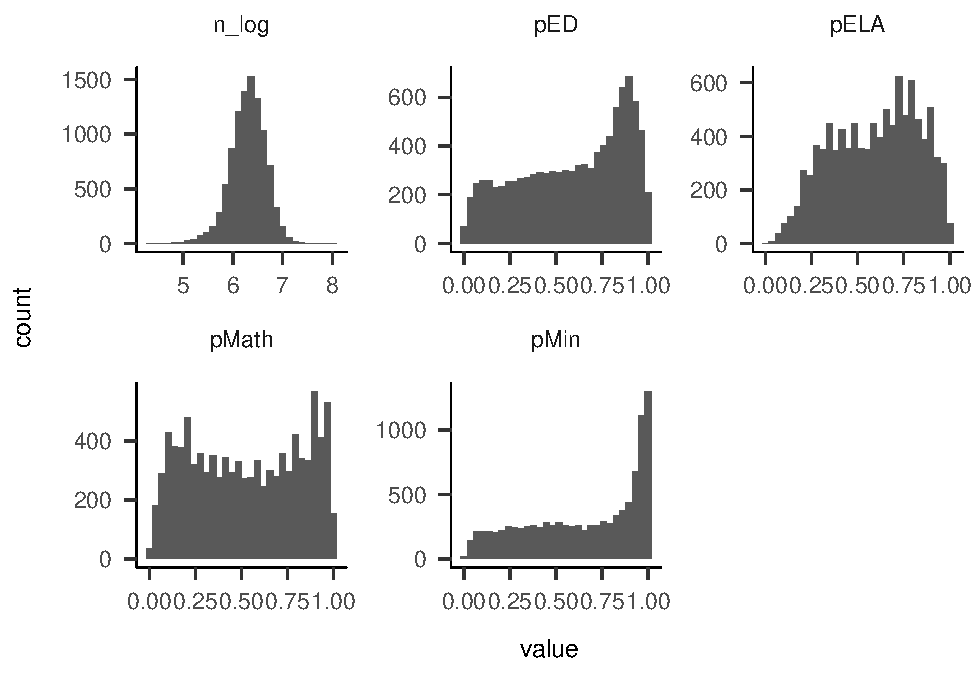
\includegraphics{GenSamp_Paper_files/figure-latex/plot-dist1-1.pdf}
\caption{\label{fig:plot-dist1}Comparison of covariate distributions and
their log transformations.}
\end{figure}

\begin{figure}
\centering
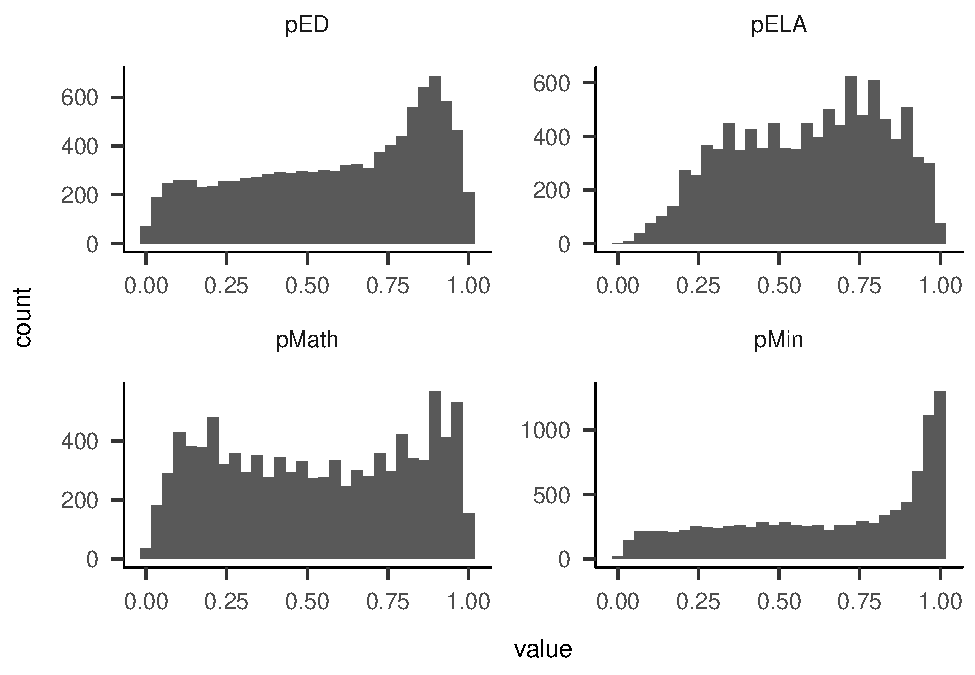
\includegraphics{GenSamp_Paper_files/figure-latex/plot-dist2-1.pdf}
\caption{\label{fig:plot-dist2}Distributions of the remaining continuous
covariates.}
\end{figure}

\hypertarget{participation-propensity-score}{%
\subsubsection{Participation Propensity
Score}\label{participation-propensity-score}}

A response generating model (RGM) was developed to simulate self
selection. The RGM creates a propensity score for each school that
indicates the probability of the school agreeing to participate if
targeted by any of the sampling method. This model assumes that schools
can be recruited directly by researchers.

Let and \(\pi^S\) be the participation propensity score. The following
base model will be used for the RGM:

\begin{align} \label{eq:sRGM}
  \log\bigg(\frac{\pi^S}{1-\pi^S}\bigg) = \gamma_{0} &+ \gamma_{1}X_{Suburban} + \gamma_{2}X_{Town/Rural} + \gamma_{3}X_{pELL} + \gamma_{4}X_{pED} 
  \\
  &+ \gamma_{5}X_{pMin} + \gamma_{6}X_{MedInc} + \gamma_{7}X_{ELA} + \gamma_{8}X_{Math} \nonumber
\end{align}

where \(X_{Suburban}\) indicates if the school is suburban,
\(X_{Town/Rural}\) indicates if the school is in a town or is rural,
\(X_{pELL}\) is the percentage of ELL students in the school,
\(X_{pED}\) is the percentage of ED students in the school, \(X_{pMin}\)
is the percentage of minority students in the school, and \(X_{MedInc}\)
is the average median household income in the school community,
\(X_{ELA}\) is the percentage of students in a school scoring at or
above proficiency on English language arts exams, and \(X_{Math}\) is
the percentage of students in a school scoring at or above proficiency
on math exams.

To select parameters for the RGM we first identified desireable sample
characteristics. Fellers (2017) compared 571 elementary schools that
participated in IES funded studies to the full population of U.S.
elementary schools on a set of similar covariates, and reported the
absolute standardized mean differences (SMD) between the schools that
participated and the population. Iterating across parameter values, we
generated \(\pi^S\) and computed the weighted mean as

\begin{align}
  m = \frac{\sum{(\frac{1}{\pi^S} X})}{\sum{\frac{1}{\pi^S}}}
\end{align}

where \(m\) represents the expected sample mean of a random sample for
covariate \(X\).

We then calculated SMDs between our expected sample mean and our
population as \(\frac{m - \mu}{\sigma}\) and compared them to the SMDs
reported by Fellers (2017), selecting parameter values that resulted in
the closest match. SMDs were not reported for academic outcomes (ELA,
Math) and neighborhood median income. However, anecdotal evidence
suggests that schools with higher academic performance are less likely
to participate in studies. We therefore selected .25 as the goal SMDs
for ELA and Math. Indicators of low SES have been shown to be predictive
at the district level (Stuart et al., 2017; Tipton et al., 2016) though
percentage of students receiving free/reduced lunch were shown to not be
predictive of school participation (Fellers, 2017). We therefore also
set .25 as the goal SMD for median income. In conjunction with iterating
across parameter values, intercept values were manipulated to generate
different levels of population participation rates. Since these rates
are unknown, we selected parameters for 9 levels of participation rates.
\ref{fig:fig-SMD-goal} reports the difference between our generated SMDs
and the goal SMDs for each covariate and each participation rate.
\ref{fig:fig-RGM-Pars} reports the parameter values we ultimately
selected for each covaraite and each participation rate.

\begin{figure}
\centering
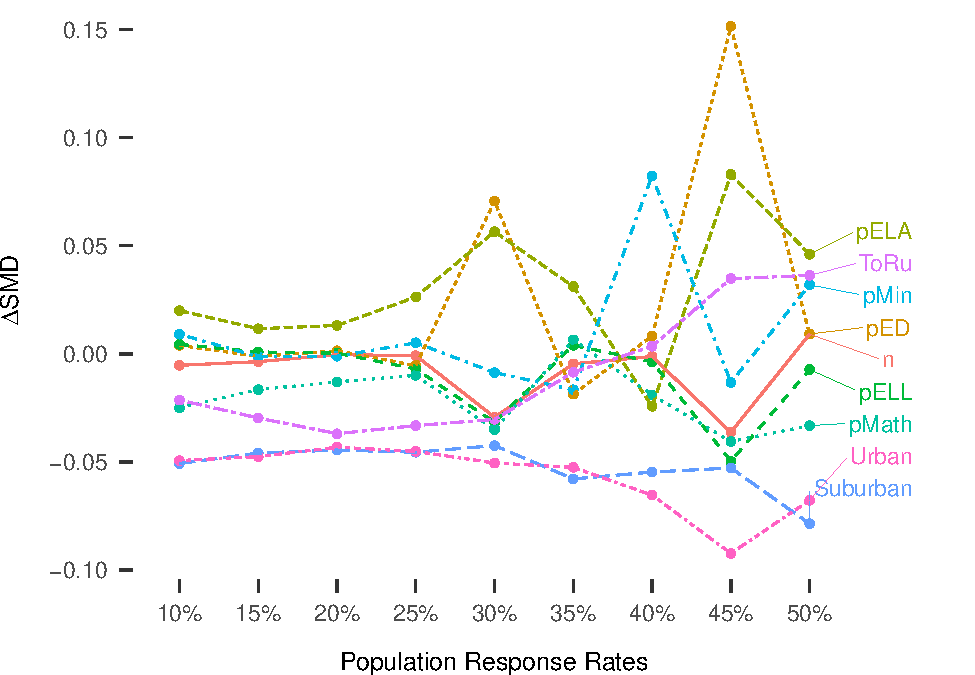
\includegraphics{GenSamp_Paper_files/figure-latex/fig-SMD-goal-1.pdf}
\caption{\label{fig:fig-SMD-goal}Difference between generated SMDs and
reported SMDs}
\end{figure}

\begin{figure}
\centering
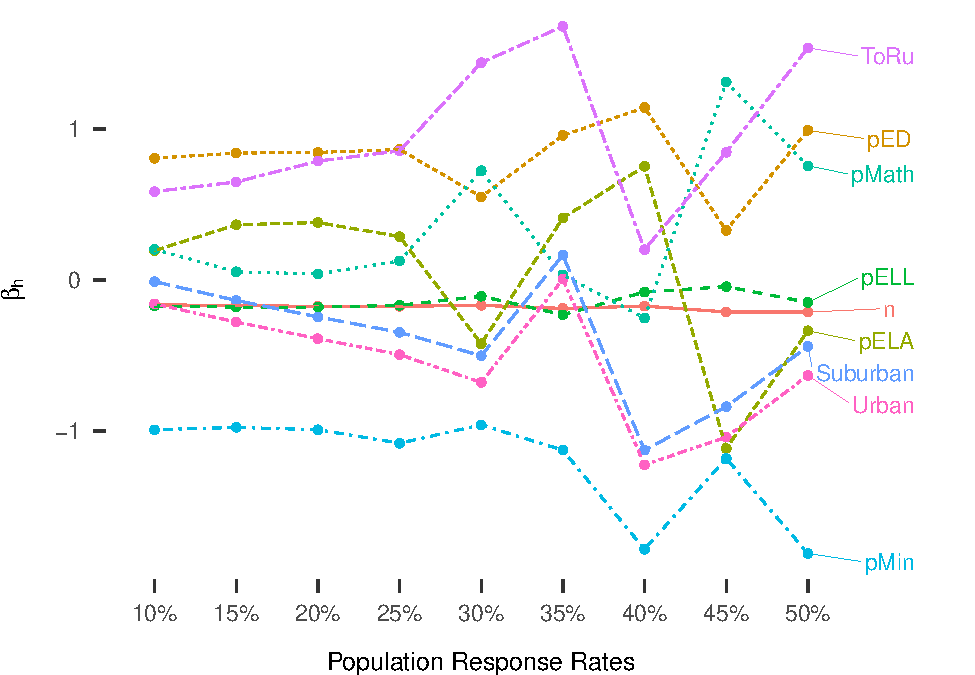
\includegraphics{GenSamp_Paper_files/figure-latex/fig-RGM-Pars-1.pdf}
\caption{\label{fig:fig-RGM-Pars}Odds ratio coeficients for Response
Generating Model}
\end{figure}

\hypertarget{stratification}{%
\subsection{Stratification}\label{stratification}}

Stratification was performed prior to simulation because the population
is constant across iterations. Per Tipton's (2013) original
recommendation, we use k-means clustering to partition the population
into strata. This requires selecting a distance metric, choosing the
number of strata, and generating the strata.

\hypertarget{distance-metric-1}{%
\subsubsection{Distance Metric}\label{distance-metric-1}}

The set of covariates include continuous variables as well as binary
indicators for urbanicity (urban, suburban, and town/rural). Within this
context it is generally recommended to use Gower's (1971) general
dissimilarity distance (Everitt, 2011; Tipton, 2013). This method relies
on different calculations of distance depending on the type of
covariates. Let \(d_{ii'h}\) be the distance between observed values of
covariate \(X_{h}\) for unit \(i\) and unit \(i'\) where \(i \ne i'\).
For categorical or dummy coded variables, \(d_{ii'h} = 1\) if
\(X_{ih} = X_{i'h}\) and \(d_{ii'h} = 0\) otherwise. For continuous
covariates, we use the following formula: \begin{align}
  d_{ii'h} = 1 - \frac{|X_{ih} - X_{i'h}|}{R_h}
\end{align} where \textbar{}.\textbar{} indicates absolute value,
\(X_{ih}\) and \(X_{i'h}\) are values of the \(h^{th}\) covariate for
units \(i\) and \(i'\), and \(R_h\) is the range of observations for
covariate \(X_h\). This method restricts the range of \(d_{ii'h}\) to
{[}0,1{]}. Finally, we calculate the general similarity between each
unit pair by taking the weighted average of the distances between all
covariates. Let \(d^{g}_{ii'}\) be the general similarity between unit
\(i\) and unit \(i'\) where \(i \ne i'\).

\begin{align}
  d^{g}_{ii'} = \frac{\sum^p_{h = 1}w_{ii'h}d_{ii'h}}{\sum^p_{h = 1}w_{ii'h}}
\end{align} where \(w_{ii'h} = 0\) if \(X_h\) is missing for either unit
and \(w_{ii'h} = 1\) otherwise. This produces an \(n\) by \(n\) distance
(or dissimilarity) matrix.

\hypertarget{number-of-clusters}{%
\subsubsection{Number of Clusters}\label{number-of-clusters}}

Selecting the number of clusters, \(k\), is one of the most difficult
problems in cluster analysis (Steinley, 2006). To date, the most
extensive investigation of methods for determining \(k\) was conducted
by Milligan and Cooper (1985) who analyzed 30 methods. However, aside
from the limited generalizability of this study, many methods are also
inappropriate in the context of non-hierarchical clustering and thus do
not support k-means clustering. Tipton (2013) states that both
statistical and practical criteria should be used in selecting the
number of clusters. For instance, a large number of clusters would
result in more homogeneous strata and, in turn, a more robust sample.
However as strata become smaller, they also become more difficult to
adequately sample from. Hennig and Liao (2013) argue that the method of
selecting \(k\) should depend on the context of the clustering and frame
the issue as one of obtaining an appropriate subject-matter-dependent
definition of rather than a statistical estimation. Ultimately three
considerations were used to select the number of clusters: the ratio of
variability between clusters to the sum of within and between cluster
variability as recommended by Tipton (2013), a generalized form of the
Calinski-Harabasz index (Calinski and Harabasz, 1974) proposed by Hennig
and Liao (2013), and the practicality of sampling from fewer clusters.

\begin{figure}
\centering
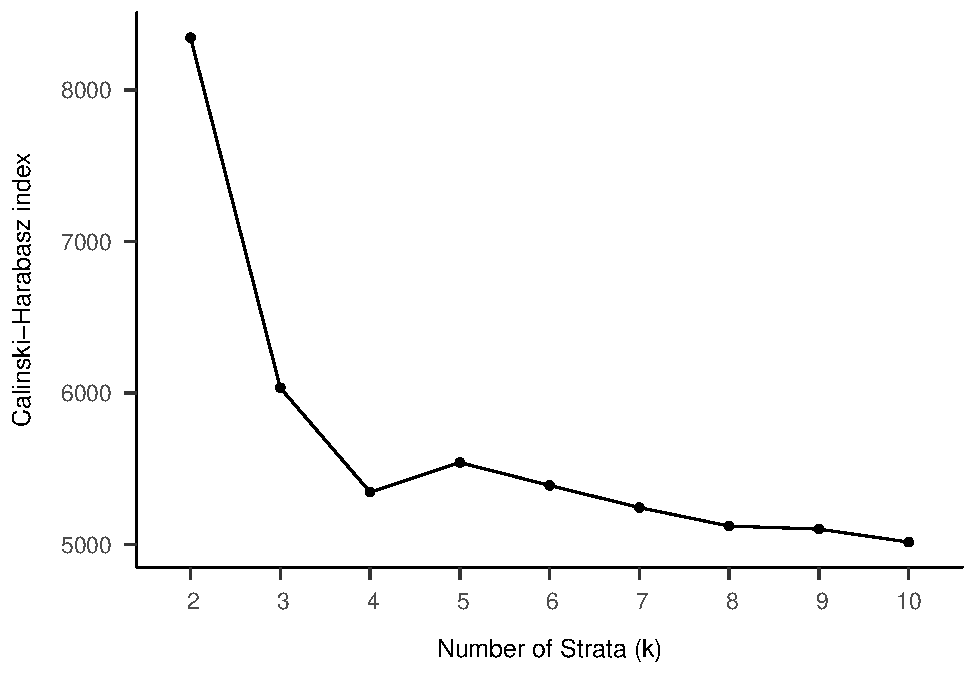
\includegraphics{GenSamp_Paper_files/figure-latex/fig-ch-1.pdf}
\caption{\label{fig:fig-ch}Generalized Calinski-Harabasz index}
\end{figure}

\begin{figure}
\centering
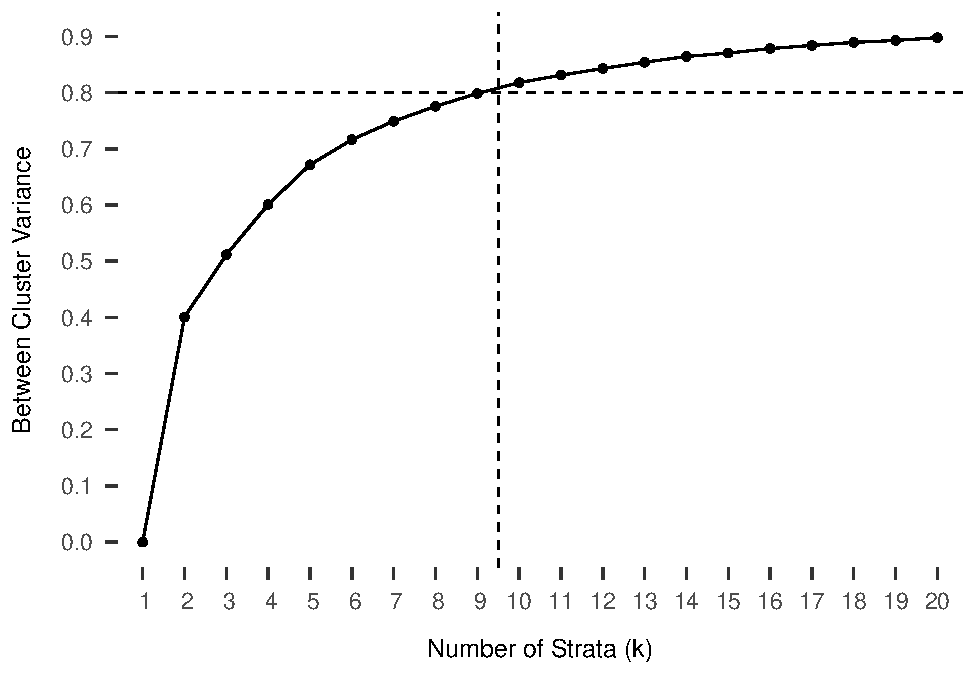
\includegraphics{GenSamp_Paper_files/figure-latex/fig-ratio-1.pdf}
\caption{\label{fig:fig-ratio}Ratio of between cluster sum of squares to
total cluster sum of squares}
\end{figure}

\begin{figure}
\centering
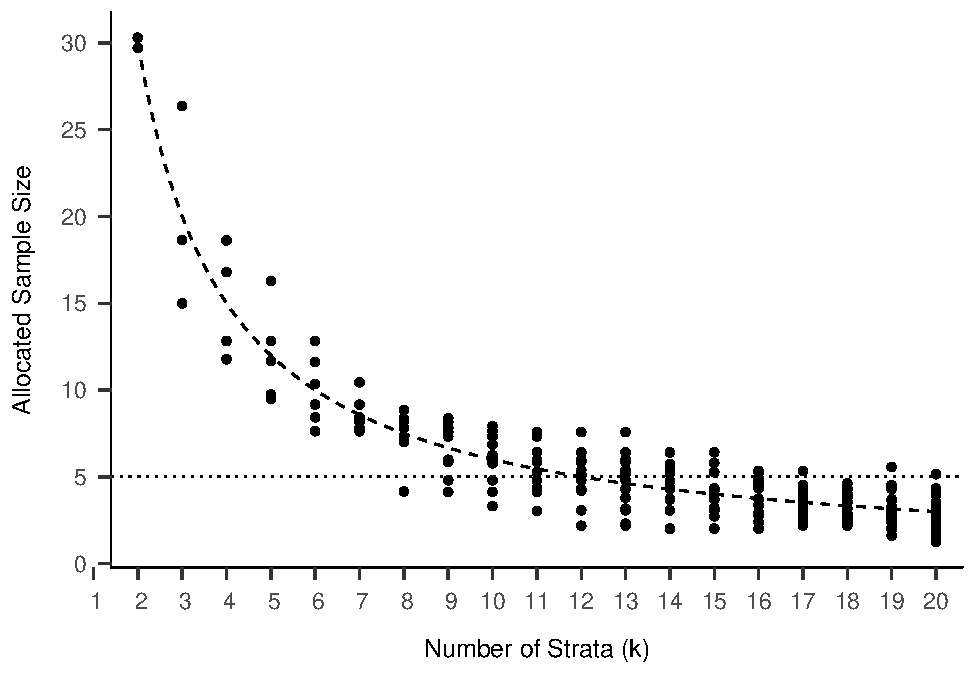
\includegraphics{GenSamp_Paper_files/figure-latex/fig-k-size-1.pdf}
\caption{\label{fig:fig-k-size}Sampling requirements for each cluster}
\end{figure}

\hypertarget{cluster-analysis}{%
\subsubsection{Cluster Analysis}\label{cluster-analysis}}

Cluster analysis was performed using the \emph{cluster} package
(Maechler et. al.~2017) in R. First, the \emph{daisy} function is used
to compute an \(n\) by \(n\) pairwise distance matrix across all
observations. This function requires two parameters: (1) the data
matrix, and (2) the distance metric. The data matrix included the full
set of school level covariates. The metric was set to \enquote{gower}.
Next the \emph{kmeans} function was used to generate clusters. This
method uses an optimization algorithm to classify units into \(k\)
clusters by minimizing the total within cluster sum of squares. This
function also requires two parameters: (1) the distance matrix, and (2)
the number of clusters to generate (\(k\)). For each \(k\), it is
recommended to run \emph{kmeans} at least 10 times, and select the
clustering that results in the smallest total within-cluster sum of
squares. {[}Get Citation{]}

Several methods were used to determine \(k\). Figure \ref{fig:fig-ch}
displays the Calinski-Harabasz (CH) index for each \(k\) clusters
generated. The value of \(k\) that maximizes the CH index should be
selected. However we see several local maxima: \(k = [2, 6, 10, 13]\).
Figure \ref{fig:fig-ratio} displays the ration of between-cluster SS to
within-cluster SS and plots it against \(k\). Tipton (2013) recommends
selecting the number of clusters such that at least 80\% of the
variability is between clusters, indicated by the figure as a dashed
line. Given this criteria it seems that at least 10 clusters should be
generated. However we also see that after a sharp initial increase, the
slope of the graph begins to level out. This indicates that as we
increase the number of clusters, the benefit of doing so decreases,
while the difficulty of sampling from each cluster increases. In that
case after 6 or 7 clusters the difficulty of sampling may not be worth
such small increases in homogeneity within clusters.

Figure \ref{fig:fig-k-size} plots the sample size that needs to be
selected from each cluster to fulfill the proportional allocation
requirement such that the number of units sampled from each cluster is
proportional to the size of the cluster in the population. The dashed
line indicates the ideal allocation if all clusters were of equal size.
We see that when 8 or less clusters are generated, they are more equally
sized, with the exception of 3 and 6 clusters where one is much larger
than the others. A sensible cutoff may be determined by looking at the
size of the smallest cluster. At \(k > 7\) it seems that the smallest
clusters would require less than 5 units being sampled, which may be
very difficult in a practical setting. Ultimately 6 clusters were
genereated.

\hypertarget{sampling-methods}{%
\subsection{Sampling Methods}\label{sampling-methods}}

Five sampling methods were compared: stratified and unstratified random
sampling (SRS, URS), stratified and unstratified convenience sampling
(SCS, UCS), and stratified balanced sampling (SBS). For all five
methods, the decision of whether or not a school agrees to participate
is the same and was generated at the start of every iteration. Let \(J\)
be the total number of schools in the population, and let schools be
indexed by \(j = 1, ..., J\). We define \(E_j\) as a binary indicator
that school \(j\) will agree to participate if contacted by recruiters,
where \(E_j = 1\) if the school agrees, and \(E_j = 0\) if the school
refuses. Each school was checked for approval by sampling from a
Bernoulli distribution with probability equal to \(\pi^S_j\) for each
school \(j\)

\begin{align} \label{eq:Ej}
  E_j \sim B(\pi^D_j)
\end{align}

To select a sample, ranks were generated for each school representing
the order in which they are approached for recruitment. Schools were
sorted by rank, with the all schools up to and including the 60th school
where \(E_j = 1\) were considered \enquote{sampled}. Ranks were
determined by the sampling method implemented.

\hypertarget{balanced-sampling}{%
\subsubsection{Balanced Sampling}\label{balanced-sampling}}

SBS is unique in that rankings are directly related to school
characteristics and do not change across iterations. Ranks within strata
are based on equation \eqref{eq:euclid}, where schools that are closer to
the \enquote{center} of the strata are more representative of it.
Schools will be ranked within strata such that \(r_k= 1\) for the school
that is most representative of strata \(k\). The percent of the total
sample recruited from each strata should be proportional to the
percentage the population of schools that are in the strata
(proportional sample allocation). Therefore, schools will be approached
independently within each strata in order of rank until the proportional
sample allocation requirements are met:
\begin{align} \label{eq:rankCASS}
  \sum_{r_{k}=1}^{R_k}{Z_{r_k} = [\frac{n_k}{N}60}]
\end{align} where \(n_k\) is the total number of schools in the strata,
\(N\) is the total number of schools in the population, and \(R_k\) is
the total number of schools approached in strata \(k\) with brackets
indicating rounding to the nearest whole number. Though extremely
unlikely, several schools and/or districts may have the same rank. In
such cases, schools with equal rank will be ordered randomly.

\hypertarget{random-sampling}{%
\subsubsection{Random Sampling}\label{random-sampling}}

In URS, a simple random sample was taken of all the schools in the
population. In the context of educational MRTs, this sampling method is
impractical. Large subsets of schools are likely to be overlooked if
samples are too small, while schools that are sampeld would be randomly
scattered throughout the state making data collection and treatment
implementation logistically difficult. More effective methods would be
clustered randomization, stratified random sampling, or some combination
of both. However, the goal here is to uses URS as a high standard for
comparison purposes. To achieve this, the order in which schools are
approached was indexed by rank, \(r\), where \(r = 1\) if a school is
approached first. Rank was randomized such that each school has an equal
probability of being approached. Once schools are ranked, each school
was approached until 60 schools agree to be in the sample:
\begin{align} \label{eq:rankRS}
  \sum_{r=1}^R{Z^S_r} = 60
\end{align} where \(R\) is the total number of schools approached. This
method allowed tracking of the number of schools that declined to
participate, \(R - 60\). For SRS, the same procedure was repeated
independantly within strata generated by the cluster analysis.
Proportional allocation was used to determine the number of schools to
select from each strata.

\hypertarget{convenience-sampling}{%
\subsubsection{Convenience Sampling}\label{convenience-sampling}}

In UCS we assume that recruiters have some knowledge of the schools'
likelihoods of participating, and prioritize recruitment based on that
knowledge in order to minimize effort. To achieve this, schools were
selected one at a time, without replacement, and assigned sequential
ranks. Schools were selected with a probability equal to
\(\frac{\pi^S}{\sum\pi^S}\) such that schools with a higher \(\pi^S\)
were more likely to receive a higher rank. Once a school was selected
and assigned a rank, the next school was selected with a probability
proportional to the weights of the remaining schools. Once all ranks
were assigned, schools were again approached until 60 schools agreed to
be in the sample:

\begin{align} \label{eq:rankCS}
  \sum_{r^S=1}^R{Z^S_{r^S} = 60}
\end{align}

As with SRS, in SCS this was performed independantly within strata, and
proportional allocation was used to set the target strata sample size.

\hypertarget{analysis}{%
\subsection{Analysis}\label{analysis}}

\hypertarget{generalizability}{%
\subsubsection{Generalizability}\label{generalizability}}

There are several methods to determine how generalizable a sample is to
a target population. One common method is to compare the sample to the
population on a range of covariates by examining SMDs. Let \(X^r_j\) be
the full set of covariates identified in Table \ref{tab:desc} indexed by
\(j = 1,...,9\) to the order of \(r\) where \(r = 1,..,3\) if \(X_j\) is
continuous and \(r = 1\) if \(X_j\) is binary. Let \(\bar{X^r_j}\) and
\(M^r_j\) be the mean of covariate \(X^r_j\) in the sample and
population respectively. Finally, let \(\sigma^r_j\) be the standard
deviation of \(X^r_j\) in the population. We will calculated the \(SMD\)
of each covariate as \begin{align}
  SMD^r_{j} = \frac{\bar{X}^{r}_{j}-M^{r}_{j}}{\sigma_{j}}
\end{align}

This method is limited as it only provides us with a measure of how
close the sample means are to the population means. To have true
generalizability, sample variance must also be representative of the
population variance. Therefore, in addition to SMDs we also estimated
the generalizability index (\(B\); Tipton, 2014). The generalizability
index is bounded between 0 and 1, with 0 indicating no overlap between
the sample and the population, and 1 indicating the sample is
representative of the population. First all units in the population are
divided into \(k\) bins. For bins \(j = 1,...,k\), let
\(w_{pj} = N_j/N\) be the proportion of the population and
\(w_{sj} = n_j/n\) be the proportion of the sample in each bin. We will
calculate \(B\) as: \begin{align}
  B = \sum^k_{j=1}\sqrt{w_{pj}w_{sj}}
\end{align} Bins must be defined such that
\(\sum{w_{pj}} = \sum{w_{sj}} = 1\). Selecting the correct number of
bins is important, as too many bins will underestimate the similarity
between distributions, and too few will overestimate. Tipton (2014)
recommends generating equal bins of size \(h\) calculated as
\begin{align}
  h = 1.06s(N+n)^{-1/5}
\end{align} where \(s^2\) is the pooled variance across the sample and
population: \begin{align}
  s^2 = \frac{(n - 1)s^2_s + (N + 1)s^2_p}{(N + n - 2)}
\end{align}

\hypertarget{feasibility}{%
\subsubsection{Feasibility}\label{feasibility}}

In order to assess feasibility, the total number of schools approached
to achieve a full sample was tracked. The average number of refusals
each sample method resulted in prior to selecting the full sample was
calculated across replications. Recruiters expend a lot of resources
contacting districts and schools, scheduling meetings and traveling
between interested locations. A project with limited resources may not
be able to afford to go through a large list of potentially uninterested
units. This measure allows us to compare the difficulty with which a
full sample is recruited using each method.

\hypertarget{results}{%
\section{Results}\label{results}}

\newpage

\hypertarget{references}{%
\section{References}\label{references}}

\begingroup
\setlength{\parindent}{-0.5in}
\setlength{\leftskip}{0.5in}

\hypertarget{refs}{}
\leavevmode\hypertarget{ref-fellersDevelopingApproachDetermine2017}{}%
Fellers, L. (2017). \emph{Developing an approach to determine
generalizability: A review of efficacy and effectiveness trials funded
by the Institute of Education Sciences} (Ph.D.). Columbia University,
United States -- New York. Retrieved from
\url{https://search.proquest.com/docview/1865595768/abstract/40FD82F4A0C24535PQ/1}

\leavevmode\hypertarget{ref-gowerGeneralCoefficientSimilarity1971}{}%
Gower, J. C. (1971). A General Coefficient of Similarity and Some of Its
Properties. \emph{Biometrics}, \emph{27}(4), 857--871.
doi:\href{https://doi.org/10.2307/2528823}{10.2307/2528823}

\leavevmode\hypertarget{ref-grovesSurveyMethodology2004}{}%
Groves, R. M. (Ed.). (2004). \emph{Survey methodology}. Hoboken, N.J:
Wiley-Interscience.

\leavevmode\hypertarget{ref-hennigHowFindAppropriate2013}{}%
Hennig, C., \& Liao, T. F. (2013). How to find an appropriate clustering
for mixed-type variables with application to socio-economic
stratification: How to Find an Appropriate Clustering. \emph{Journal of
the Royal Statistical Society: Series C (Applied Statistics)},
\emph{62}(3), 309--369.
doi:\href{https://doi.org/10.1111/j.1467-9876.2012.01066.x}{10.1111/j.1467-9876.2012.01066.x}

\leavevmode\hypertarget{ref-olsenExternalValidityPolicy2013}{}%
Olsen, R. B., Orr, L. L., Bell, S. H., \& Stuart, E. A. (2013). External
Validity in Policy Evaluations That Choose Sites Purposively.
\emph{Journal of Policy Analysis and Management}, \emph{32}(1),
107--121.
doi:\href{https://doi.org/10.1002/pam.21660}{10.1002/pam.21660}

\leavevmode\hypertarget{ref-omuircheartaighGeneralizingUnrepresentativeExperiments2014}{}%
O'Muircheartaigh, C., \& Hedges, L. V. (2014). Generalizing from
unrepresentative experiments: A stratified propensity score approach.
\emph{Journal of the Royal Statistical Society: Series C (Applied
Statistics)}, \emph{63}(2), 195--210.
doi:\href{https://doi.org/10.1111/rssc.12037}{10.1111/rssc.12037}

\leavevmode\hypertarget{ref-raudenbushStatisticalPowerOptimal2000}{}%
Raudenbush, S. W., \& Liu, X. (2000). Statistical power and optimal
design for multisite randomized trials. \emph{Psychological Methods},
\emph{5}(2), 199--213.
doi:\href{https://doi.org/10.1037//1082-989X.5.2.199}{10.1037//1082-989X.5.2.199}

\leavevmode\hypertarget{ref-roschelleIntegrationTechnologyCurriculum2010}{}%
Roschelle, J., Shechtman, N., Tatar, D., Hegedus, S., Hopkins, B.,
Empson, S., \ldots{} Gallagher, L. P. (2010). Integration of Technology,
Curriculum, and Professional Development for Advancing Middle School
Mathematics: Three Large-Scale Studies. \emph{American Educational
Research Journal}, \emph{47}(4), 833--878.

\leavevmode\hypertarget{ref-shadishExperimentalQuasiexperimentalDesigns2002}{}%
Shadish, W. R., Cook, T. D., \& Campbell, D. T. (2002).
\emph{Experimental and quasi-experimental designs for generalized causal
inference}. Boston, MA, US: Houghton, Mifflin and Company.

\leavevmode\hypertarget{ref-stuartCharacteristicsSchoolDistricts2017}{}%
Stuart, E. A., Bell, S. H., Ebnesajjad, C., Olsen, R. B., \& Orr, L. L.
(2017). Characteristics of School Districts That Participate in Rigorous
National Educational Evaluations. \emph{Journal of Research on
Educational Effectiveness}, \emph{10}(1), 168--206.
doi:\href{https://doi.org/10.1080/19345747.2016.1205160}{10.1080/19345747.2016.1205160}

\leavevmode\hypertarget{ref-stuartUsePropensityScores2011}{}%
Stuart, E. A., Cole, S. R., Bradshaw, C. P., \& Leaf, P. J. (2011). The
use of propensity scores to assess the generalizability of results from
randomized trials: Use of Propensity Scores to Assess Generalizability.
\emph{Journal of the Royal Statistical Society: Series A (Statistics in
Society)}, \emph{174}(2), 369--386.
doi:\href{https://doi.org/10.1111/j.1467-985X.2010.00673.x}{10.1111/j.1467-985X.2010.00673.x}

\leavevmode\hypertarget{ref-tiptonImprovingGeneralizationsExperiments2013}{}%
Tipton, E. (2013a). Improving Generalizations From Experiments Using
Propensity Score Subclassification: Assumptions, Properties, and
Contexts. \emph{Journal of Educational and Behavioral Statistics},
\emph{38}(3), 239--266. Retrieved from
\url{https://www.jstor.org/stable/41999424}

\leavevmode\hypertarget{ref-tiptonStratifiedSamplingUsing2013}{}%
Tipton, E. (2013b). Stratified Sampling Using Cluster Analysis: A Sample
Selection Strategy for Improved Generalizations From Experiments.
\emph{Evaluation Review}, \emph{37}(2), 109--139.
doi:\href{https://doi.org/10.1177/0193841X13516324}{10.1177/0193841X13516324}

\leavevmode\hypertarget{ref-tiptonHowGeneralizableYour2014}{}%
Tipton, E. (2014). How Generalizable Is Your Experiment? An Index for
Comparing Experimental Samples and Populations. \emph{Journal of
Educational and Behavioral Statistics}, \emph{39}(6), 478--501.

\leavevmode\hypertarget{ref-tiptonSiteSelectionExperiments2016}{}%
Tipton, E., Fellers, L., Caverly, S., Vaden-Kiernan, M., Borman, G.,
Sullivan, K., \& de Castilla, V. R. (2016). Site Selection in
Experiments: An Assessment of Site Recruitment and Generalizability in
Two Scale-up Studies. \emph{Journal of Research on Educational
Effectiveness}, \emph{9}(sup1), 209--228.
doi:\href{https://doi.org/10.1080/19345747.2015.1105895}{10.1080/19345747.2015.1105895}

\leavevmode\hypertarget{ref-tiptonImplicationsSmallSamples2017}{}%
Tipton, E., Hallberg, K., Hedges, L. V., \& Chan, W. (2017).
Implications of Small Samples for Generalization: Adjustments and Rules
of Thumb. \emph{Evaluation Review}, \emph{41}(5), 472--505.
doi:\href{https://doi.org/10.1177/0193841X16655665}{10.1177/0193841X16655665}

\endgroup


\end{document}
